\documentclass{unn}

%%%%%%%%%%%%%%%%%%%%%%%%%%%%%%%%%%%%%%%%%%%%%%%%%%%%%%%%%%%%%
% Настройки титулки
\usepackage{review-titlepage}
\TitleWorkTitle{
  Метод компенсации нелинейных искажений усилителя
  мощности для стандарта мобильной связи 5G NR 
}

\setauthor{1}{}{Шиков А.П.}
%%%%%%%%%%%%%%%%%%%%%%%%%%%%%%%%%%%%%%%%%%%%%%%%%%%%%%%%%%%%%

\usepackage{booktabs} % For \toprule, \midrule and \bottomrule
\usepackage{siunitx} % Formats the units and values
\usepackage{pgfplotstable} % Generates table from .csv
\pgfplotsset{compat=1.18}
\usepackage{tabularx}
% Setup siunitx:
\sisetup{
  round-mode          = places, % Rounds numbers
  round-precision     = 2, % to 2 places
}


\addbibresource{library.bib}
\usepackage{enumitem}
\usepackage{subcaption}
\usepackage{soulutf8}

\makeatletter
\patchcmd{\@setref}{\bfseries ??}{\bfseries\hl{??}}{}{}
\makeatother
% \pagenumbering{gobble}



\begin{document}
\maketitle
\newpage
\Introduction

Развитие стандарта мобильной связи 5G New Radio (NR), разрабатываемого консорциумом
3GPP (\textit{Англ. - 3rd Generation Partnership Project}), тесно связано с развитием
технологии Интернета Вещей (\textit{Англ. - IoT - Internet of Things}). Высокая скорость,
надежность сети, малая задержка, а также возможность массового подключения
"умных" устройств являются важнейшими параметрами, определяющими
производительность системы в целом.

Одни из последних релизов стандарта 5G NR - релизы 15 и 16 обеспечивают
поддержку несущих частот до 52.6 ГГц. С целью расширить поддержку текущего
частотного диапазона FR2 (\textit{Англ. - Frequency Range 2}) до 52.6 - 71 ГГц с
минимальными вносимыми изменениями в систему \cite{intel193259}
\cite{qlcm193229}, группа RAN проекта 3GPP уже исследовала требования для
диапазона 52.6 - 114.25 ГГц \cite{3gpp.38.807}. Помимо этого, была также
исследована возможность расширения частотного диапазона до миллиметровых
волн 71-114 ГГц. Однако в этом диапазоне появляется такое ограничение, как
нелинейный искажения, вызванные работой усилителя мощности (УМ). Несмотря
на значительное продвижение в технологии разработки и проектирования УМ с
использованием новых материалов, все ещё наблюдаются значительные нелинейные
искажения сигнала при использовании стандартной мощности передатчика
\cite{zhang2021}. В данном диапазоне частот УМ может внести значительные
искажения, кардинально снизив производительность
системы. Это особенно заметно для высокоэффективных модуляций, например,
64-QAM и 256-QAM.

Данным эффектом искажения сигнала можно пренебречь в низких диапазонах
частот, таких как FR1 и частично FR2. Рабочую точку УМ в этих диапазонах
можно выбрать таким образом, что на выходе усилителя будет достигаться
необходимая выходная мощность, и при этом УМ будет работать в линейной
области своей характеристики, что минимизирует вносимые в передаваемый
сигнал искажения.


Проблема компенсации нелинейных искажений, вносимых УМ, рассматривалась во
многих работах, в том числе для низких диапазонов частот
\cite[]{sharath2015,shabany2008,eda2001,maltsev2021,bhat2016,qi2010,gregorio2007}.
Рассматривались различные подходы, в основе которых лежали предварительное
искажение (\textit{Англ. - Pre-Distortion (PD), Digital Pre-Distortion
(DPD)}) сигнала на передатчике с целью "выпрямления" амплитудной
характеристики усилителя. Однако такие методы требуют дополнительной
сигнальной обработки на передатчике, что негативно влияет на
энергоэффективность устройства. В основе другого метода лежит обработка
сигнала на приемнике, когда принятый сигнал подвергается обработке на
стороне принимающего устройства с целью компенсации искажений, внесенных на
УМ передатчика. В качестве методов компенсации используют обратную
характеристику УМ, статистические подходы для определения усредненного
искажения и его дальнейшей компенсации, последовательный метод Монте-Карло
и другие. Также важно отметить необходимость в определенных случаях знать
на приемнике параметры УМ, который расположен на передатчике.

Также важно отметить, что характеристики УМ в миллиметровом диапазоне
частот 100-200 ГГц значительно отличаются от характеристик усилителей в
диапазоне 30-70 ГГц. На более высоких частотах, характеристики значительно
хуже, это означает необходимость применения определенного метода
компенсации искажения для повышения качества передачи информации.

\section{Описание искажений вносимых нелинейным усилителем мощности}
Для описания искажения амплитуды и фазы при использовании твердотельных УМ
широко используется модель Раппа (\textit{Англ. - Rapp}) \cite{Rapp1991} \cite{Maltsev2010}.
Также существует модифицированная модель Раппа, приведенная в выражении
\ref{eq:Rapp}. Данная модель УМ включена в список моделей в спецификации
3GPP \cite{3gpp.38.803}.

\begin{equation}
    F_{AM/AM}(x) = \frac{G x}{\left( 1 + \abs{\frac{Gx}{V_{sat}}}^{2p}\right)^{1/2p}},
    \quad 
    F_{AM/PM}(x) = \frac{Ax^q}{\left(1+\left(\frac{x}{B}\right)^q\right)},
    \label{eq:Rapp}
\end{equation}
где $F_{AM/AM}, F_{AM/PM}$ - амплитудные и фазовые характеристики
соответственно, $G$ - КУ слабого сигнала, $V_{sat}$ - амплитуда насыщения,
$p$ - показатель гладкости характеристики. Параметры $A,B,q$ - параметры
кривой искажения фазы.

\begin{figure}[h!]
  \centering
  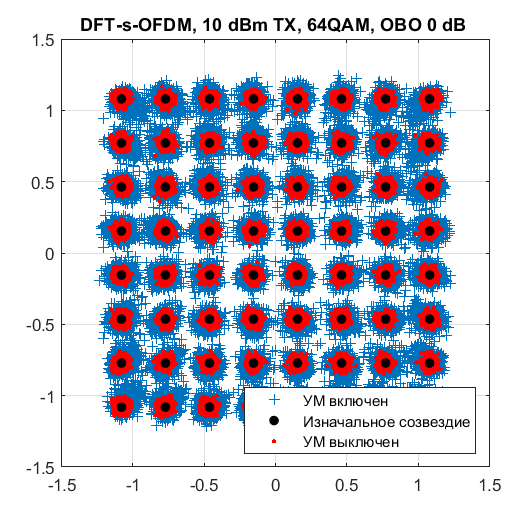
\includegraphics[width=0.35\linewidth]{figs/dfts_10dbm_obo0.png}
  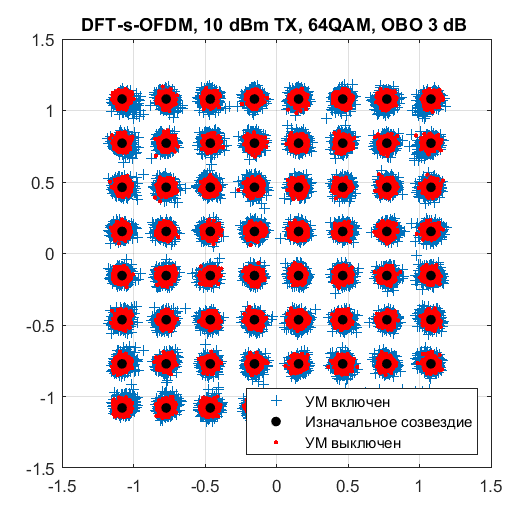
\includegraphics[width=0.35\linewidth]{figs/dfts_10dbm_obo3.png}
  \caption{Демонстрация искажения созвездий на приемнике в результате
  использования нелинейного УМ с выходной мощностью 10 dBm в LLS. На левом
  графике $OBO=0$ dB, на правом - $OBO=3$ dB.}
  \label{fig:lls_rapp_distortions_10dbm}
\end{figure}

На приемнике, в результате внесенных изменений наблюдаются искажения
полученных созвездий. Пример таких искажений в случае
использования сигнала DFT-s-OFDM при $P^{dBm}_{TX} = 10$ dBm, $OBO = 0,3$
dB, $SNR=30$ dB и использовании модуляции 64-QAM приведен на рис.
\ref{fig:lls_rapp_distortions_10dbm}. В качестве модели УМ использовалась
модель Раппа \ref{eq:Rapp}, с параметрами приведенными в \cite{nokia163314}.


\section{Обзор существующих методов борьбы с нелинейными искажениями усилителя мощности}
На текущий момент были исследованы несколько основных подходов для
компенсации нелинейных искажений, они разделяются на два основных
направления — обработка на передатчике, либо приемнике.

\subsection{Обработка сигнала на передатчике}

Первый метод заключается в предварительном искажении сигнала перед
подачей на УМ на передатчике. Сигналу придаются свойства, которые
минимизируют влияние нелинейного искажения от УМ, эффективно "выпрямляя"
его АХ. Существует множество вариантов обработки для данного подхода,
однако многие из них имеют слабый эффект на общей производительности
системы, а подход с применением предварительного искажения сигнала имеет
низкую эффективность при низких значениях IBO, при которой достигается
максимальная эффективность усилителя \cite{sharath2015}
\cite{shabany2008} \cite{eda2001}. Также, использование PD на передатчике
нежелательно на малогабаритных устройствах, поскольку в таком случае
увеличивается сложность устройства, объем сигнальной обработки и энергопотребление.

\subsection{Обработка сигнала на приемнике}

Второй основной подход заключается в компенсации нелинейных искажений на
приемнике. Например, в работе \cite{maltsev2021} используется
статистическая обработка принятого сигнала для определения степени
искажения, на основе которой в дальнейшем производится компенсация. Многие
работы \cite[]{sharath2015, shabany2008,bhat2016,qi2010,gregorio2007,
bouhadda2015,drotar2010} рассматривают теоретический подход для компенсации
на приемнике в очень обобщенном случае. Несколько методов компенсации были
предложены для OFDM сигнала \cite[]{gregorio2007,bouhadda2015, drotar2010},
где влияние нелинейности представляется комплексным множителем, а также
Гауссовой шумовой компонентой. Основной задачей в таком случае является
определение параметров УМ (они могут быть как известны изначально, так и
определены с помощью пилотных сигналов) для компенсации нелинейного
искажения. Несколько методов были исследованы для сигнала SC с одной несущей
(\textit{Англ. - SC - Single Carrier}) \cite[]{sharath2015,
shabany2008,bhat2016, qi2010}, в частности использовалась обратная
характеристика УМ и последовательные методы Монте-Карло. В нескольких
случаях \cite[]{bhat2016, qi2010,gregorio2007}, значения параметров УМ
считаются известными на приемнике, что позволяет произвести компенсацию
искажения. В случаях, когда параметры УМ оцениваются, производительность
такая же либо хуже.

\section{Краткое описание и содержание работы}
В работе изучается влияние нелинейности УМ на производительность
системы. Для описания работы усилителя использовалась модель Раппа для
диапазона 30-70 ГГц. Также была разработана усредненная модель для
диапазона 100-200 ГГц. 

Использование нелинейного УМ приводит к значительным искажениям сигналов
CP-OFDM и DFT-s-OFDM. В результате при декодировании принятого сигнала
возникают ошибки, понижающие эффективность работы системы. При
использовании модели 100-200 ГГц искажения носят более сильный характер.
Возникает необходимость компенсации внесенных искажений. Обработка возможна
на передатчике или приемнике, однако для минимизации нагрузки на передающее
устройство использование компенсации на приемнике предпочтительнее.

В работе описывается новый метод компенсации нелинейных искажений внесенных
усилителем мощности на приемнике для двух типов сигнала - CP-OFDM и
DFT-s-OFDM. Основа метода заключается в применении обработки, эквивалентной
обработке на передатчике для переноса сигнала во временную область, где
сигнал искажался усилителем, а также применении ограниченной обратной
амплитудной характеристики усилителя на основе известных параметров для
компенсации искажений. Рассматривается применение метода для различных
типов сигнала.


\section{Заключение}
В работе было изучено влияние искажений нелинейного усилителя на
эффективность работы системы. Так же была разработана модель усилителя для
диапазона 100-200 ГГц. Описан и протестирован метод компенсации искажений
на приемнике, адаптируемый в зависимости от используемого сигнала. Метод
продемонстрировал возможность улучшить результат работы системы для числа
случаев, основное преимущество метода заключается в обработке на приемнике,
что минимизирует нагрузку на передатчик.

\newpage
{\footnotesize
\printbibliography
}


\end{document}


